\documentclass{article}

% If you're new to LaTeX, here's some short tutorials:
% https://www.overleaf.com/learn/latex/Learn_LaTeX_in_30_minutes
% https://en.wikibooks.org/wiki/LaTeX/Basics

% Formatting
\usepackage[utf8]{inputenc}
\usepackage[margin=1in]{geometry}
\usepackage[titletoc,title]{appendix}

% Math
% https://www.overleaf.com/learn/latex/Mathematical_expressions
% https://en.wikibooks.org/wiki/LaTeX/Mathematics
\usepackage{amsmath,amsfonts,amssymb,mathtools}

% Images
% https://www.overleaf.com/learn/latex/Inserting_Images
% https://en.wikibooks.org/wiki/LaTeX/Floats,_Figures_and_Captions
\usepackage{graphicx,float}
\usepackage{pdfpages}

% Tables
% https://www.overleaf.com/learn/latex/Tables
% https://en.wikibooks.org/wiki/LaTeX/Tables

% Algorithms
% https://www.overleaf.com/learn/latex/algorithms
% https://en.wikibooks.org/wiki/LaTeX/Algorithms
\usepackage[ruled,vlined]{algorithm2e}
\usepackage{algorithmic}

% Code syntax highlighting
% https://www.overleaf.com/learn/latex/Code_Highlighting_with_minted
\usepackage{minted}
\usemintedstyle{borland}

% References
% https://www.overleaf.com/learn/latex/Bibliography_management_in_LaTeX
% https://en.wikibooks.org/wiki/LaTeX/Bibliography_Management
\usepackage[backend=biber, style=authoryear]{biblatex}
\addbibresource{myBibliography.bib}

% Title content
\title{AMATH 582 Homework 2}
\author{Daniel Burnham (https://github.com/burnhamdr)}
\date{February 09, 2020}

\begin{document}

\maketitle

% Abstract
\begin{abstract}
The work presented here is motivated by material covered in AMATH 582 Computational Methods For Data Analysis regarding signal time-frequency analysis. For signals recorded in time it is often desirable to understand not just the frequency content of the entire signal, but also how that frequency content changes over the time course of the signal. This can be addressed through implementation of the G\'abor transform which is a method for extracting the frequency spectrum from a signal at sequential time steps. This report will highlight the methods of application for this time-frequency analysis approach through analysis of two different sets of audio recordings of music. The first analyzed audio sample is a 9 second sample of the Hallelujah chorus from Handel's Messiah. With this example audio data different G\'abor transform filters will be explored, and their effects on the time-frequency analysis results will be characterized. The second part of the report will focus on results obtained from the time-frequency analysis of two separate recordings of a piano and a recorder performing Marry Had a Little Lamb. From the results of the Ga\'bor transform applied to these audio recordings the musical notes will be extracted. Overall, a key idea illustrated through this work is the trade off between accurately localizing a frequency in time versus resolving the frequency band of the signal for a specific time bin. This time-frequency resolution trade off will be discussed in greater detail throughout the following report.
\end{abstract}

% Introduction and Overview
\section{Introduction and Overview}
Time-frequency analysis is useful for determining when certain frequencies occur within a signal that evolves in time. Audio signals are an example of such a signal, as the sounds that make up the signal occur at individual frequencies and isolated moments in time. The specific audio signals used in this work are the Hallelujah chorus from Handel's "Messiah", and "Mary had a Little Lamb" performed on the piano and the recorder. To extract information about how the frequency spectrum of an audio recording evolves in time, G\'abor transforms are applied to each audio signal utilizing various time bin sizes and filter shapes. Experimenting in this way allowed for the advantages and disadvantages of G\'abor transformation time-frequency analysis to be visualized. 

Spectrograms are a used to visualize the frequency versus time behavior of the G\'abor transformed signal while varying properties of the time filtering window. Additional plots are also generated to demonstrate the action of the time filtering window on the signal at successive time steps. From these visualizations the musical score of the piano and recorder renditions of "Mary Had a Little Lamb" were determined.

%  Theoretical Background
\section{Theoretical Background}
The main concept explored with this work is the implementation of the G\'abor transform. The G\'abor transform is a modification of the Fourier transform kernel aimed at allowing for frequencies to be localized in time. The G\'abor transform kernel is shown in Equation~\ref{eqn:gaborKernel}(\cite{kutz_2013}).
\begin{equation}
g_{t,w}(\tau) = e^{i\omega\tau}g(\tau - t)
    \label{eqn:gaborKernel}
\end{equation}

The G\'abor transform is also known as the short-time Fourier transform (STFT) and is thus defined similarly to the FFT as representing a function as a sum of cosines and sines Equation~\ref{eqn:gaborTransform}(\cite{kutz_2013}).
\begin{equation}
    G[f](t,\omega) = \tilde{f}_{g}(t,\omega) = \int_{-\infty}^{\infty}f(\tau)g(\tau - t)e^{i\omega\tau}d\tau
    \label{eqn:gaborTransform}
\end{equation}
The purpose of the function $g(\tau - t)$ is to establish a window centered at $t = \tau$ outside of which the signal is damped to zero. Shifting this window across the signal in time thus allows for sections of the signal to be analyzed for frequency content. Various window functions can be used. For example, in this work we experiment with the following window functions (\cite{kutz_2013}):
\begin{align}
    g(t) = e^{-at^2} &\quad \mathrm{(Gaussian)} \\
	g(t) = (1 - at^{2})e^{-\frac{t^{2}}{2}} &\quad \mathrm{(Mexican~Hat)} \\
	g(t) = 
				\begin{cases}
					0 & |t|>1/2 \\
					1 & |t|\leq 1/2
				\end{cases}	&\quad \mathrm{(Shannon)}
\end{align}

The G\'abor method using these sliding windows trades away
accuracy in either the time or frequency domains in order
to provide a measurement of both time and frequency resolution simultaneously. In performing this windowed signal filtering, signal components with periods longer than the window will not be represented in the frequency spectrum. This limitation is at the heart of the time-frequency resolution trade off where to localize a frequency one must select a shorter time bin to filter, however, this results in the loss of information on low frequency signal components.

\subsection{Spectrogram}
A spectrogram is a heat map plot of time versus frequency where the intensity of the indicated heat illustrates the amplitude of the frequency bands at each time interval. The spectrogram is generated by first applying the G\'abor transform utilizing a filter of interest across the signal. Then, the frequency spectrum data for each time bin is plotted against the time points where the G\'abor filters were centered. This results in a heat map of frequency bands indicating the frequency content of the signal as extracted by the G\'abor filter at the time points of interest.

% Algorithm Implementation and Development
\section{Algorithm Implementation and Development}
The main steps of the algorithm are as follows: 
\begin{enumerate}
    \item Input the audio file, prepare for analysis
    \item Generate desired G\'abor filter
    \item Plot the signal multiplied by the filter to demonstrate the action of the modified Fourier Transform kernel. Also plot frequency spectrum at sequential time bins.
    \item Take the Fourier Transform to generate the frequency spectrum of the signal after G\'abor filtering at each time step.
    \item Plot the spectrogram to illustrate the frequency content of the signal for each time bin.
\end{enumerate}

% Computational Results
\section{Computational Results}
\subsection{Part I: Handel Music G\'abor Transforms}
See Figure~\ref{fig:gaussFilt}, Figure~\ref{fig:mexFilt}, and Figure~\ref{fig:shanFilt} for examples of applying the G\'abor method using a Gaussian, Mexican Hat, and Shannon function filter respectively. More in depth analysis is delineated in the attached code where different filter widths and different $d\tau$ values are tested to investigate the impacts on the signal spectrogram. The filters shown in Figure~\ref{fig:gaussFilt}, Figure~\ref{fig:mexFilt}, and Figure~\ref{fig:shanFilt} are examples of instances where oversampling is achieved because the widths of the filters allowed for overlap in the signal extracted by each successive filter shift. Oversampling ensures that good resolution in time and frequency is achieved.

% begin{figure}[tb] % t = top, b = bottom, etc.
\begin{figure}
    \centering
    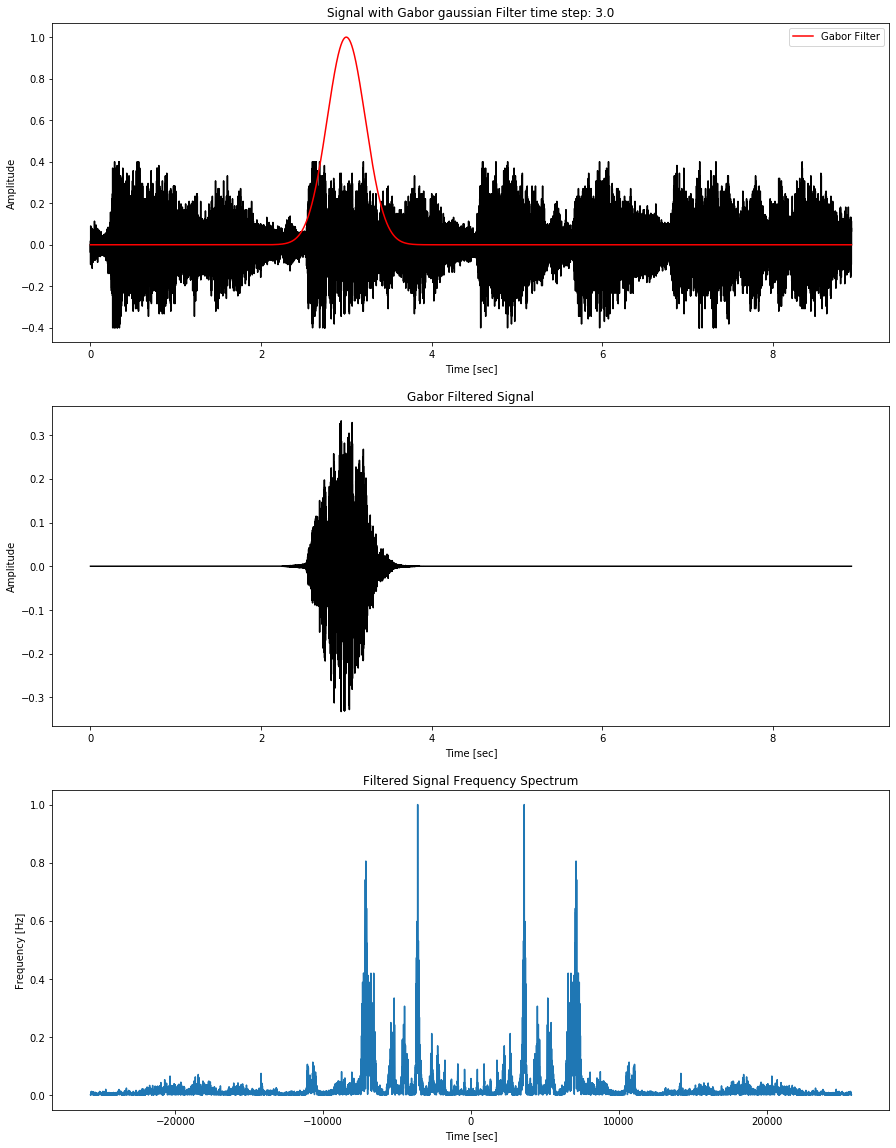
\includegraphics[width=0.435\linewidth]{HW2_DanielBurnham_files/HW2_DanielBurnham_5_2.png}
    \caption{Example of the action of the G\'abor method using a standard Gaussian filter for one time bin ($d\tau = 0.1$) within the signal. The top plot shows the complete signal with the filter overlaid. The middle plot shows the result of applying the filter to the signal. The bottom plot is the frequency spectrum of the filtered signal content.}
    \label{fig:gaussFilt}
\end{figure}

\begin{figure}
    \centering
    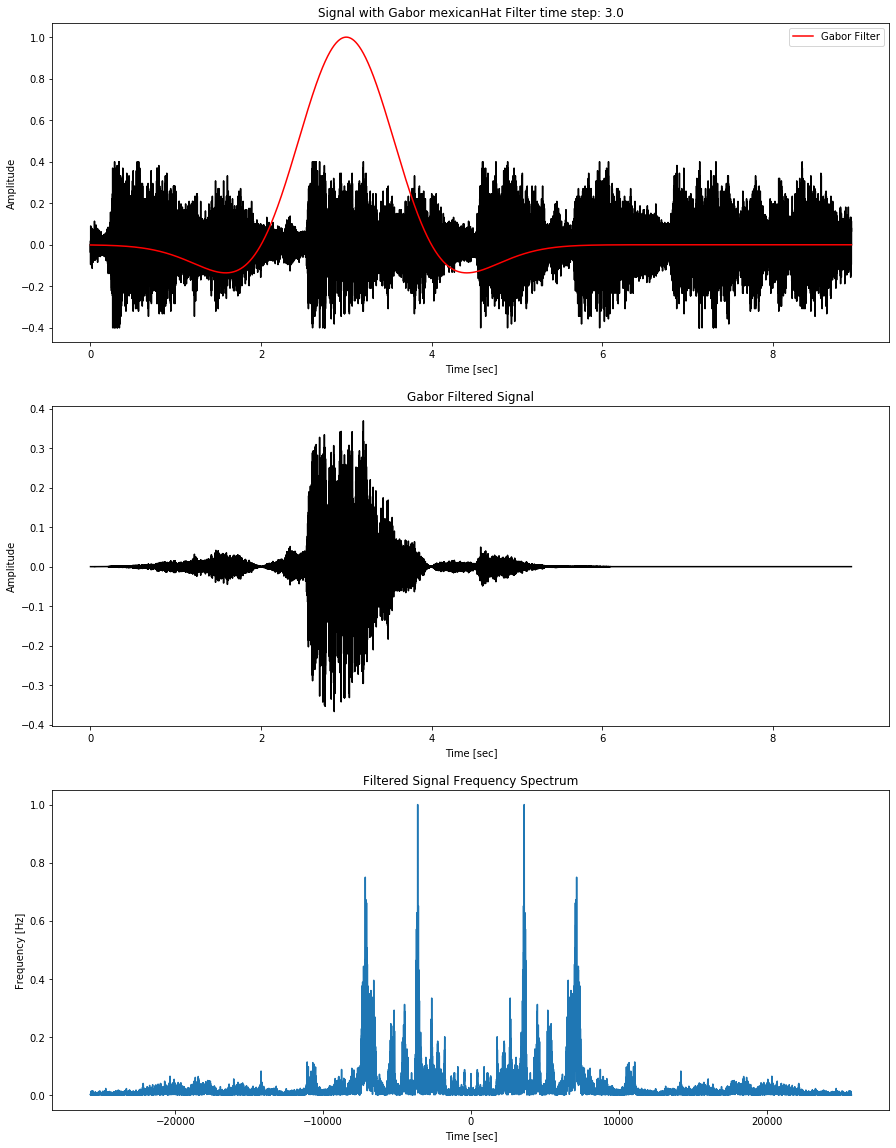
\includegraphics[width=0.435\linewidth]{HW2_DanielBurnham_files/HW2_DanielBurnham_7_2.png}
    \caption{Example of the action of the G\'abor method using a Mexican Hat filter for one time bin ($d\tau = 0.1$) within the signal. The top plot shows the complete signal with the filter overlaid. The middle plot shows the result of applying the filter to the signal. The bottom plot is the frequency spectrum of the filtered signal content.}
    \label{fig:mexFilt}
\end{figure}
\begin{figure}
    \centering
    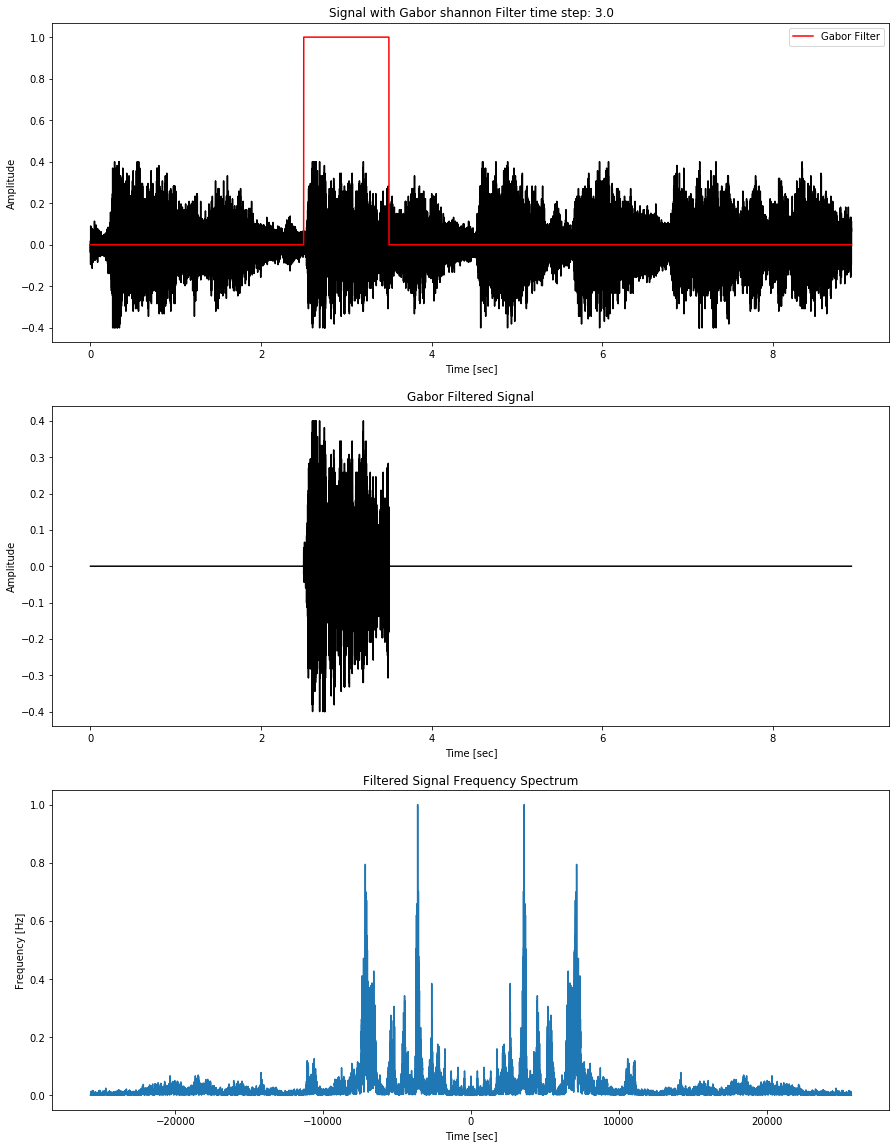
\includegraphics[width=0.435\linewidth]{HW2_DanielBurnham_files/HW2_DanielBurnham_10_2.png}
    \caption{Example of the action of the G\'abor method using a Shannon filter for one time bin ($d\tau = 0.1$) within the signal. The top plot shows the complete signal with the filter overlaid. The middle plot shows the result of applying the filter to the signal. The bottom plot is the frequency spectrum of the filtered signal content.}
    \label{fig:shanFilt}
\end{figure}

The spectrograms for the G\'abor Transforms utilizing the filters depicted in Figure~\ref{fig:gaussFilt}, Figure~\ref{fig:mexFilt}, and Figure~\ref{fig:shanFilt} are shown in Figure~\ref{fig:gaussSpec}, Figure~\ref{fig:mexSpec}, and Figure~\ref{fig:shanSpec} respectively. With the $d\tau$ chosen for these figures, blurring along the time axis can be observed in both the Gaussian and Mexican Hat filter instances. In contrast, the Shannon filter seems to result in a stuttering effect across time most likely caused by the sharpness of the filter boundary. In further investigation carried out in the source code (Appendix~\ref{appendix:code}) blurring of the frequency bands in time is shown to be exacerbated by filter width, and blurring of the frequency bands across frequencies is created with a sufficiently narrow filter width. This is consistent with expectations based on the theoretical understanding of the G\'abor method described earlier. If the filtering samples large sections in time, the frequency resolution will be good because longer wavelength signals can be represented in the frequency spectrum of the sample extracted by the filter. However, the temporal resolution will be poor because the time bin is large thus making it difficult to determine when the individual frequencies occur in time.

\begin{figure}
    \centering
    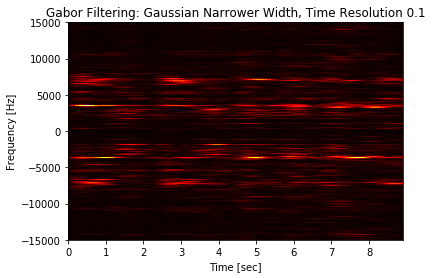
\includegraphics[width=0.7\linewidth]{HW2_DanielBurnham_files/HW2_DanielBurnham_5_6.png}
    \caption{Spectrogram illustrating the frequency content of the signal for each time bin ($d\tau = 0.1$) utilizing a Gaussian filter. The intensity of the heat map represents the scale of the amplitude of the frequency bands.}
    \label{fig:gaussSpec}
\end{figure}

\begin{figure}
    \centering
    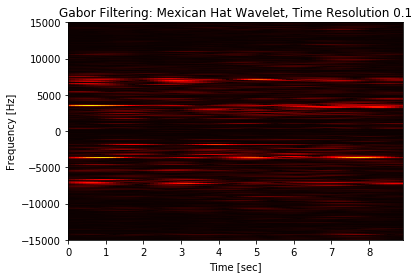
\includegraphics[width=0.7\linewidth]{HW2_DanielBurnham_files/HW2_DanielBurnham_7_6.png}
    \caption{Spectrogram illustrating the frequency content of the signal for each time bin ($d\tau = 0.1$) utilizing a Mexican Hat filter. The intensity of the heat map represents the scale of the amplitude of the frequency bands.}
    \label{fig:mexSpec}
\end{figure}
\begin{figure}
    \centering
    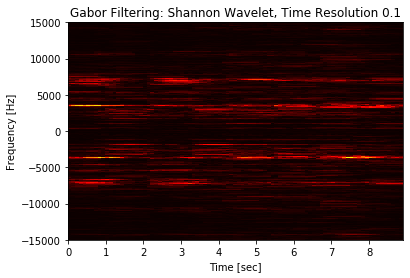
\includegraphics[width=0.7\linewidth]{HW2_DanielBurnham_files/HW2_DanielBurnham_10_6.png}
    \caption{Spectrogram illustrating the frequency content of the signal for each time bin ($d\tau = 0.1$) utilizing a Shannon filter. The intensity of the heat map represents the scale of the amplitude of the frequency bands.}
    \label{fig:shanSpec}
\end{figure}

\subsection{Part II: Piano and Recorder Music G\'abor Transforms}
The G\'abor Method for time-frequency analysis was performed similarly to Part I. A narrow Gaussian filter with a time bin width $d\tau = 0.1$ was used for the analysis. The spectrograms for the recorder (Figure~\ref{fig:recSpec}) and piano (Figure~\ref{fig:pianoSpec}) music samples of "Mary Had a Little Lamb" indicate sharp bands at the frequencies of the individual notes played. Through detection of the maximum frequency signal in each time bin and converting from wave number to frequency in Hz ($\omega = 2\pi f$), the notes in each musical score were detected and plotted in Figure~\ref{fig:recScore} and Figure~\ref{fig:pianoScore}. Overtones are faintly evident in the piano rendition spectrogram around 250 Hz.

\begin{figure}
    \centering
    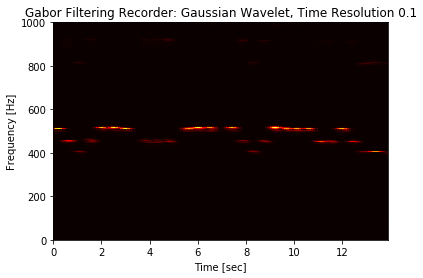
\includegraphics[width=0.75\linewidth]{HW2_DanielBurnham_files/HW2_DanielBurnham_14_7.png}
    \caption{Spectrogram illustrating the frequency content of the recorder rendition for each time bin ($d\tau = 0.1$) utilizing a Gaussian filter. The intensity of the heat map represents the scale of the amplitude of the frequency bands.}
    \label{fig:recSpec}
\end{figure}
\begin{figure}
    \centering
    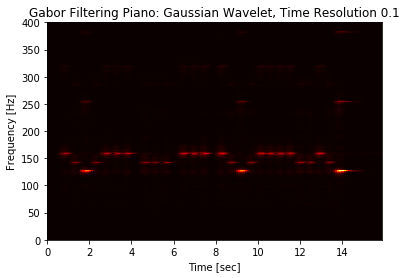
\includegraphics[width=0.75\linewidth]{HW2_DanielBurnham_files/HW2_DanielBurnham_15_7.png}
    \caption{Spectrogram illustrating the frequency content of the piano rendition for each time bin ($d\tau = 0.1$) utilizing a Gaussian filter. The intensity of the heat map represents the scale of the amplitude of the frequency bands.}
    \label{fig:pianoSpec}
\end{figure}

\begin{figure}
    \centering
    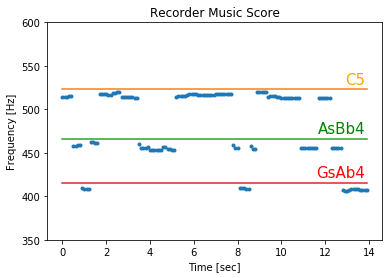
\includegraphics[width=0.75\linewidth]{HW2_DanielBurnham_files/HW2_DanielBurnham_16_1.png}
    \caption{Musical score of the recorder rendition of "Mary Had a Little Lamb"}
    \label{fig:recScore}
\end{figure}
\begin{figure}
    \centering
    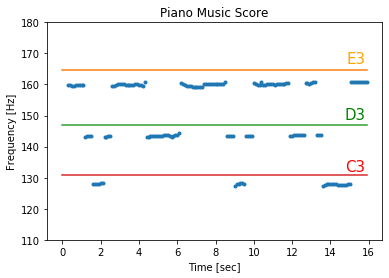
\includegraphics[width=0.75\linewidth]{HW2_DanielBurnham_files/HW2_DanielBurnham_17_1.png}
    \caption{Musical score of the piano rendition of "Mary Had a Little Lamb"}
    \label{fig:pianoScore}
\end{figure}

% Summary and Conclusions
\section{Summary and Conclusions}
In Part I the G\'abor method for performing time-frequency analysis was successfully employed and many cases were explored to illustrate the trade off between time and frequency resolution, and the qualitative characteristics of different filter shapes. Blurring in the time domain was generated by under-sampling due to a large filter window. Blurring in the frequency domain was observed when the filter window was sufficiently small as to exclude many frequencies from detection based on wavelength.

In Part II the methods practiced in Part I were implemented to determine the musical score of "Mary Had a Little Lamb" played both on the piano and on the recorder. The G\'abor method for time-frequency analysis using a narrow Gaussian filter successfully produced spectrograms illustrating bands consistent with an expected musical score. These bands were translated into musical notes by converting the wave number of the maximum frequency signature in each time bin to a temporal frequency.

% References
\printbibliography

% Appendices
\begin{appendices}

% Python Functions
\section{Python Functions}
\begin{itemize}
    \item \texttt{matplotlib.pyplot.pcolormesh(*args, alpha=None, norm=None, cmap=None, vmin=None, vmax=None, shading='flat', antialiased=False, data=None, **kwargs)[source]} Create a pseudocolor plot with a non-regular rectangular grid.
    \item \texttt{numpy.fft.fft2(a, s=None, axes=(-2, -1), norm=None)} Compute the 2-dimensional discrete Fourier Transform.
    This function computes the n-dimensional discrete Fourier Transform over any axes in an M-dimensional array by means of the Fast Fourier Transform (FFT). By default, the transform is computed over the last two axes of the input array, i.e., a 2-dimensional FFT.
    \item \texttt{numpy.fft.fftshift(x, axes=None)} returns the Shift the zero-frequency component to the center of the spectrum.
    This function swaps half-spaces for all axes listed (defaults to all). Note that y[0] is the Nyquist component only if len(x) is even.
    \item \texttt{numpy.argmin(a, axis=None, out=None)} Returns the indices of the minimum values along an axis.
    \item \texttt{numpy.argmax(a, axis=None, out=None)} Returns the indices of the maximum values along an axis.
    
\label{itemize:functions}
\end{itemize}

% Python Code
\section{Python Code}
\inputminted{python}{HW2_DanielBurnham_files/HW2_DanielBurnham_final}
\label{appendix:code}

\end{appendices}



\end{document}